% @suppress InvalidSymbol
\section{本研究のシステム}
本研究では\UTF{6FF5}野の研究で挙げられていた本人拒否率の改善を目標とする.
また,特定の図形や記号を元にしたモーションだけでなく,端末を上下に振るなどより単純で日常的な入力が容易なモーションでの利用が可能なシステムを目指す.
%システムの動作フローを図\ref{flow}に示す.

%\begin{figure}[bthp]
%    \centering
%    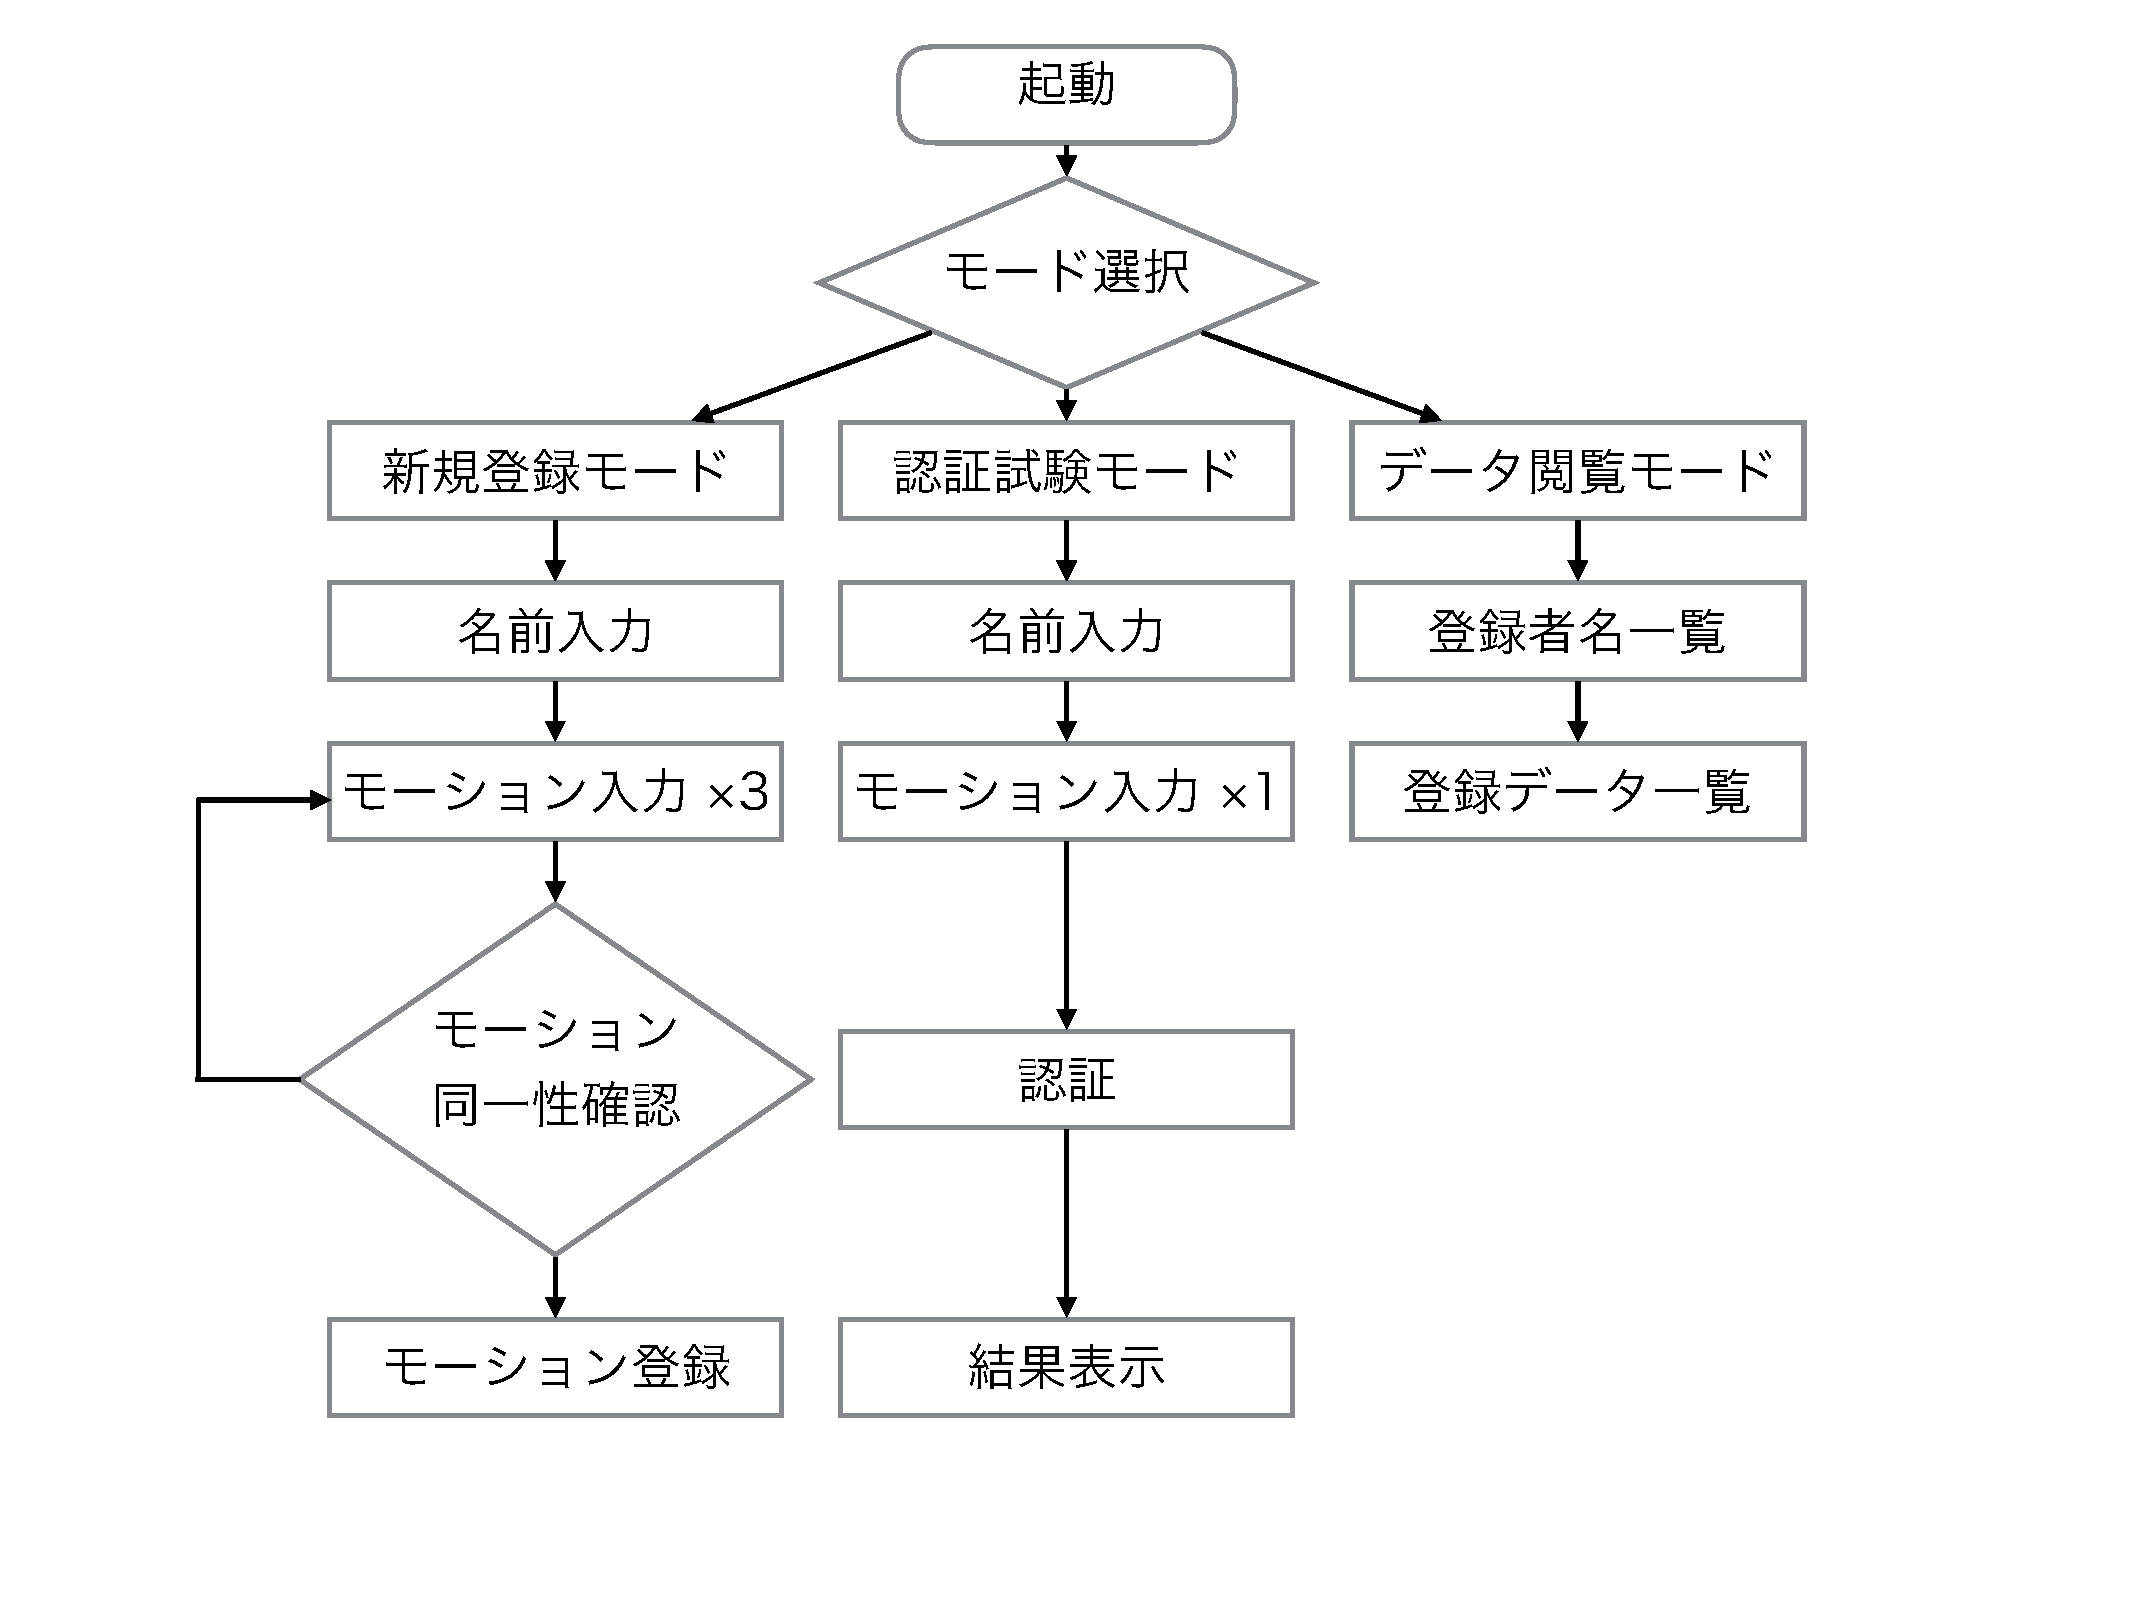
\includegraphics[bb=0 100 950 750, width=80mm]{flow.pdf}
%    \caption{システム動作フロー}
%    \label{flow}
%\end{figure}

アプリケーション起動時に表示されるモード選択ダイアログから,ユーザはまず新規登録モードを選択する.
このモードでは,ユーザ名を指定して個人認証を行う際の鍵情報となるモーションを登録できる.
モード選択後登録したいユーザ名を入力し,モーションの入力を任意の長さで3回行う.
得られたデータに対して同一モーションでの類似度の低下を防ぐ加工を施し,コサイン類似度を用いて取得したデータが同一のモーションであるかを確認する.
同一のモーションであればモーション入力時に生じうる時間的なズレを修正する.
同一のモーションでなければモーションの取り直しを行う.
時間的なズレを修正する処理を行った3回分のデータから平均値を求め,これを増幅量とともに登録する.

これらの処理を行うことで\UTF{6FF5}野の研究であげられていた認証成功率の問題に対処し,対応できるモーションの幅を広げている.

認証試験モードでは,あらかじめ新規登録モードにおいてモーションの登録を行ったユーザ名を指定する.
指定されたユーザ名で既にモーションの登録がなされていることが確認できた場合のみ,モーションの入力画面に移る.
認証試験モードでは,モーションの入力を任意の長さで1回行う.
得られたデータに対して同一モーションでの類似度の低下を防ぐ加工を施したものと,登録されたデータとのコサイン類似度を求め,個人認証を行う.

データ閲覧モードでは,新規登録モードにおいて登録されたユーザ名及びモーションデータを,リスト形式で閲覧できる.

